\documentclass[a4paper]{article}

\usepackage{pgfplots}

\pgfplotsset{compat=1.3}

\begin{document}
\parindent=0pt
\parskip=20pt

%\tracingmacros=2 \tracingcommands=2
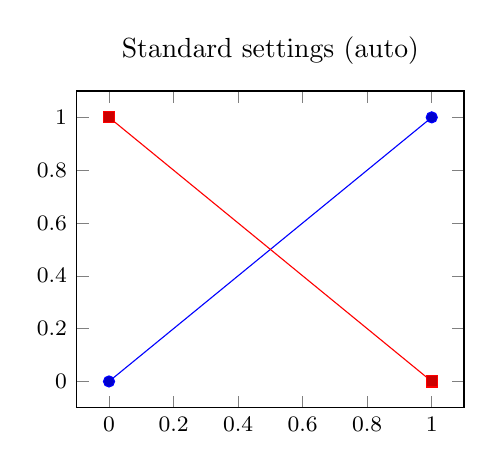
\begin{tikzpicture}
\begin{axis}[
	title=Standard settings (auto),
	small,
]
    \addplot coordinates {(0,0) (1,1)};
    \addplot coordinates {(0,1) (1,0)};
\end{axis}
\end{tikzpicture}
\message{^^J^^JSecond picture ^^J^^J}%
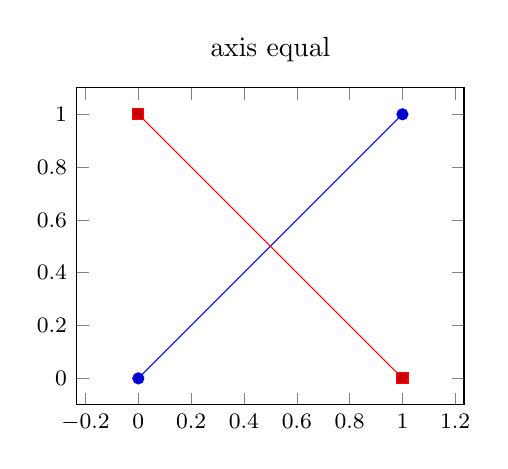
\begin{tikzpicture}
\begin{axis}[
	title=axis equal,
	axis equal,
	small]
    \addplot coordinates {(0,0) (1,1)};
    \addplot coordinates {(0,1) (1,0)};
\end{axis}
\end{tikzpicture}

\message{^^J^^JThird picture ^^J^^J}%
\pgfplotsset{small,width=5cm,height=7cm}

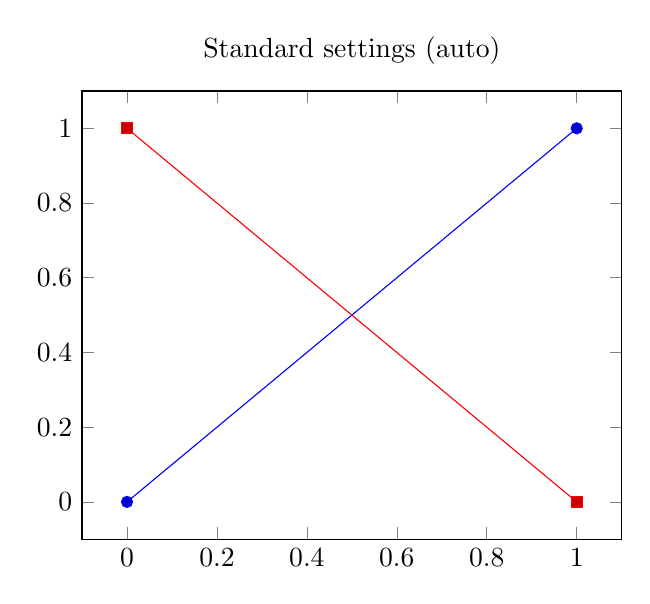
\begin{tikzpicture}
\begin{axis}[
	title=Standard settings (auto),
	%small,
]
    \addplot coordinates {(0,0) (1,1)};
    \addplot coordinates {(0,1) (1,0)};
\end{axis}
\end{tikzpicture}
\message{^^J^^JFourthh picture ^^J^^J}%
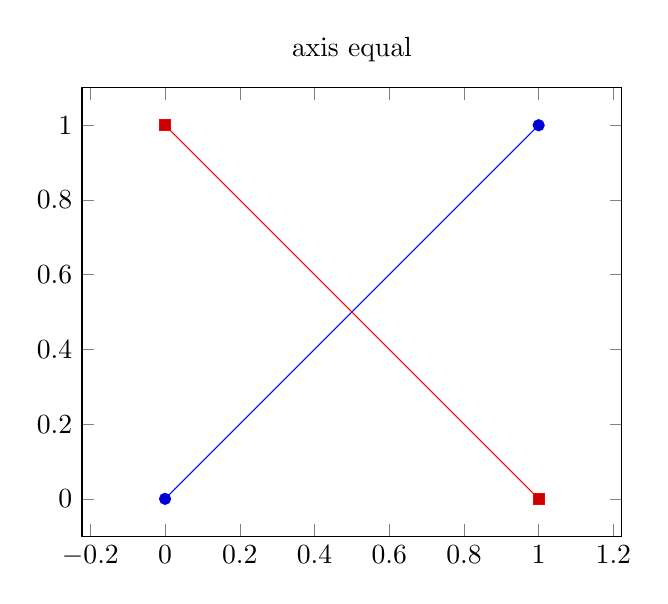
\begin{tikzpicture}
\begin{axis}[
	title=axis equal,
	axis equal,
	%small,
]
    \addplot coordinates {(0,0) (1,1)};
    \addplot coordinates {(0,1) (1,0)};
\end{axis}
\end{tikzpicture}
\end{document}

